\clearpage

\section{개요}

\subsection{목적}

본 프로젝트는 C/C++ 소스 코드의 보안 취약점을 탐지하는 AI 모델 프로토타입을 개발하여, 기존 정적 분석 도구의 구조적 한계를 해결하는 것을 목표로 한다.
기존 정적 분석 도구들은 규칙 기반 탐지에 의존함으로써 높은 False Positive Rate와 문맥 인식의 부재를 보이며, 실제 개발 현장에서 상당한 검증 비용과 피로도를 유발한다.
본 연구는 이러한 문제를 해결하기 위해 코드의 구조적 문맥 정보를 활용하는 학습 기반 접근 방식을 도입한다.

구체적으로, 소스 코드로부터 Abstract Syntax Tree(AST, 이하 \abbrAST)를 추출하여 그래프 표현으로 변환하고,
이를 Graph Neural Network(GNN, 이하 \abbrGNN)를 통한 학습으로 취약점 패턴을 인식한다.
이는 코드의 구조적 관계를 그래프 형태로 모델링함으로써, 단순 패턴 일치가 아닌 문맥을 고려한 정확한 취약점 탐지를 가능하게 한다.

\subsection{프로그램 구성 및 설계}

본 시스템은 크게 그래프 데이터 추출 단계와 GNN 기반 분류 단계로 구성된다.
첫째, 소스 코드로부터 AST 그래프를 추출하는 전처리 파이프라인을 거치고, 둘째, 추출된 AST 그래프를 GNN 모델에 입력하여 취약점 여부를 분류한다.

\subsubsection{데이터 전처리 파이프라인}

소스 코드를 GNN 학습에 적합한 그래프 표현으로 변환하기 위해 다음과 같은 단계를 거친다.

\begin{itemize}
\item \textbf{CPG 생성}: Joern을 활용하여 C/C++ 소스 코드를 \abbrCPG 로 변환한다. CPG는 코드의 구문, 제어 흐름, 타입 정보 등을 통합적으로 표현하는 멀티 계층 그래프 구조이다.
    
    \item \textbf{Template 변환}: CPG의 복잡한 구조를 정규화하여 템플릿 그래프로 변환한다. 이 과정에서 연산자 이름 정규화(\texttt{<operator>.addition} $\rightarrow$ \texttt{+}), 제어 구조 표준화, 타입 추론 등이 수행된다. 이렇게 정규화된 템플릿 그래프는 이후 단계를 통해 기계 학습에 직접 활용 가능한 \abbrAST 기반 그래프 표현으로 변환된다.
    
    \item \textbf{AST 추출}: 템플릿 그래프에서 AST 구조만을 추출하여 계층적 트리 형태로 재구성한다. AST 추출 모듈은 이를 평탄화된 문장 수준 그래프로 변환하며, Parent-Child, Sibling, Guard 세 가지 유형의 엣지를 생성하여 구조적 관계를 보존한다.
    
    \item \textbf{특징 벡터 생성}: 각 노드에 대해 노드 타입, 루프 컨텍스트, 가드 조건, 호출 의미 등 GNN 학습에 필요한 수치형 특징 벡터를 계산한다.
\end{itemize}

\subsubsection{GNN 기반 분류 파이프라인}

추출된 AST 그래프를 입력으로 받아 취약점을 탐지하는 과정은 다음과 같다.

\begin{itemize}
\item \textbf{그래프 인코딩}: AST 그래프를 \abbrGINE\ 인코더에 통과시켜 노드별 임베딩 벡터를 생성한다. \abbrGINE 은 그래프의 구조적 특성과 엣지 속성을 동시에 고려하여 노드 표현을 학습한다.
    
    \item \textbf{그래프 수준 표현}: Global Mean Pooling을 통해 노드별 임베딩을 집계하여 전체 그래프를 하나의 고정 길이 벡터로 변환한다. 이 그래프 임베딩 벡터는 함수 전체의 구조적 패턴을 요약한다.
    
    \item \textbf{분류}: 그래프 임베딩 벡터를 선형 분류기에 입력하여 해당 함수가 Vulnerable 인지 Safe 인지를 이진 분류한다. 학습 단계에서는 레이블링된 데이터셋을 사용하여 모델 파라미터를 최적화하고, 추론 단계에서는 학습된 모델을 사용하여 새로운 함수의 취약점 여부를 판별한다.
\end{itemize}

전체 파이프라인은 Figure~\ref{fig:program-flow}에 도식화되어 있다.

\begin{figure}[H]
    \centering
    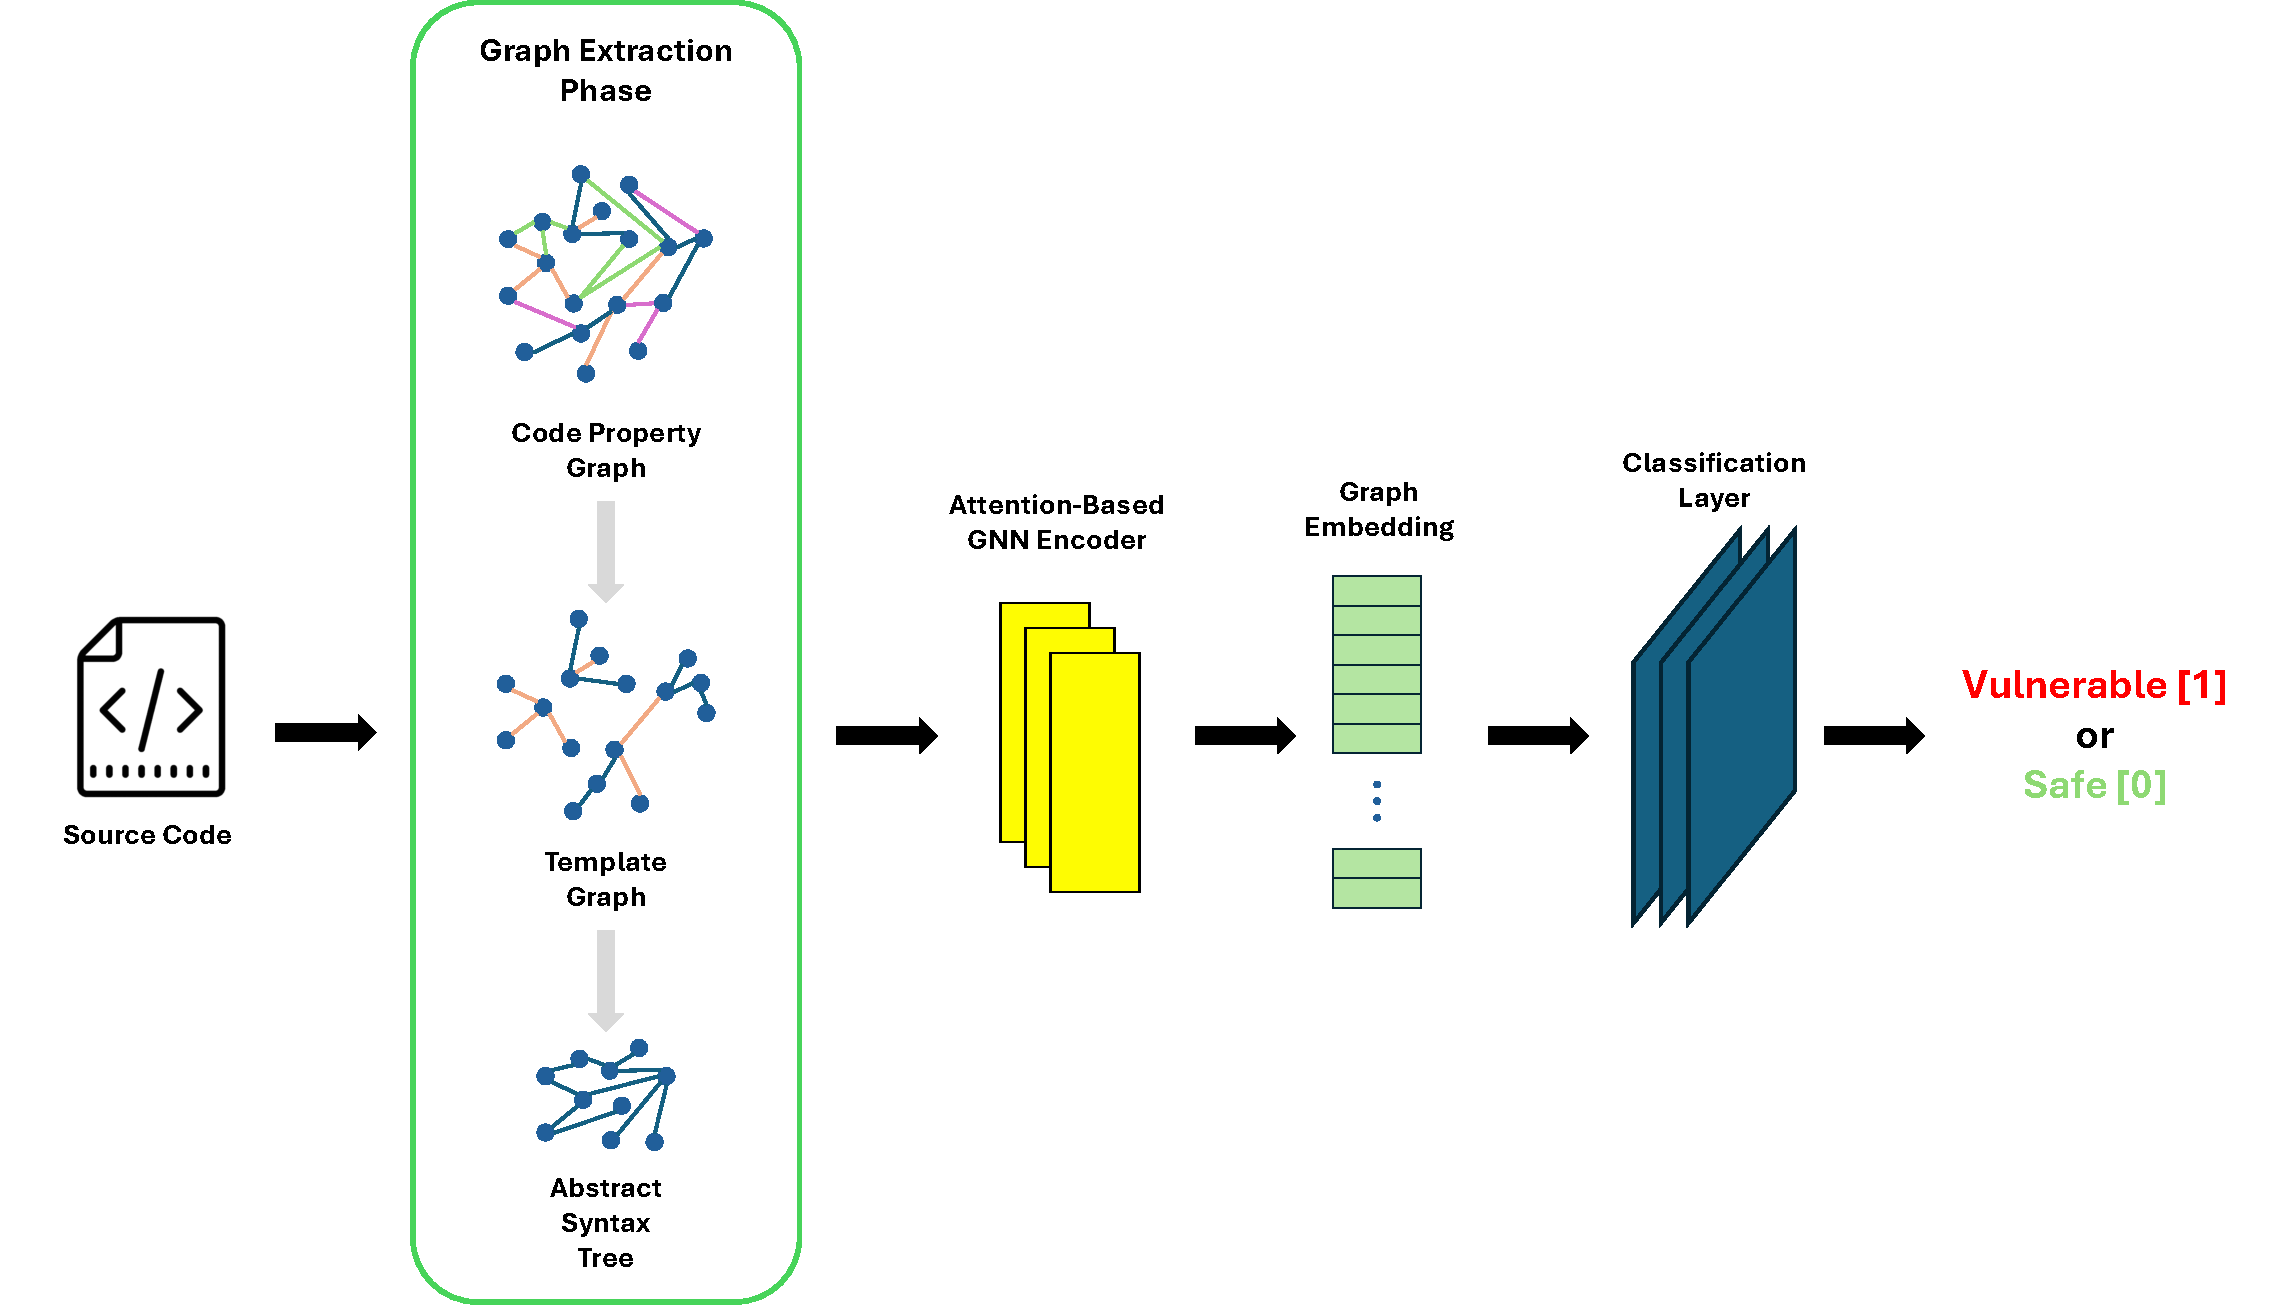
\includegraphics[width=\textwidth]{overall-process.pdf}
    \caption{프로그램 전체 흐름 구성도}
    \label{fig:program-flow}
\end{figure}